\subsection{Arduino}
\noindent Initial interfacing to the sensors was performed using the Arduino integrated development environment. Because of its ease of access and abstraction, this has become the preferred programming tool for the FORWARD system. The Arduino IDE can 

\subsection{Detection Subsystem}
\noindent Recall the requirements of the detection subsystem. It should be able to detect objects at least 3 meters away and within a 15 degree aspect angle. It also should detect walker instability up to 10 degrees in pitch angle. It should detect hazards with an accuracy of at least 80\%. Finally, feedback latency should not exceed 100 milliseconds to keep the user safe.\\

\noindent Let us also define the input and output of the obstacle detection subsystem. The input is energy return from the environment, supplied to 5 different points on the walker frame, as well as accelerometer and magnetometer data outputs describing the attitude of the walker itself. The output is somewhat joint with the obstacle identification system, as it helps to generate velocity motor commands for both speed and turn angle. Detection and identification are the FORWARD system inputs, and avoidance is the output.

\subsubsection{Sensor Orientation}
\noindent The range sensors are mounted on the frame perpendicularly to obstacles. In other words, the direction of the energy transmitted is perpendicular to the ground. However, the question of maximizing capability of detecting obstacles at the wheel level, and to prevent ignorance of more dangerous and deceptive hazards such as ledges or step-downs is raised. The monostatic ones will be mounted on the legs near the wheels, front-facing. These

\subsubsection{Incline and Decline Stability}
\noindent The simple function fulfilled by the inclusion and integration of the IMU is stability. By monitoring the pitch angle of the walker, we know whether the user is at risk of falling over.\\

\begin{figure}[H]
	\centering
	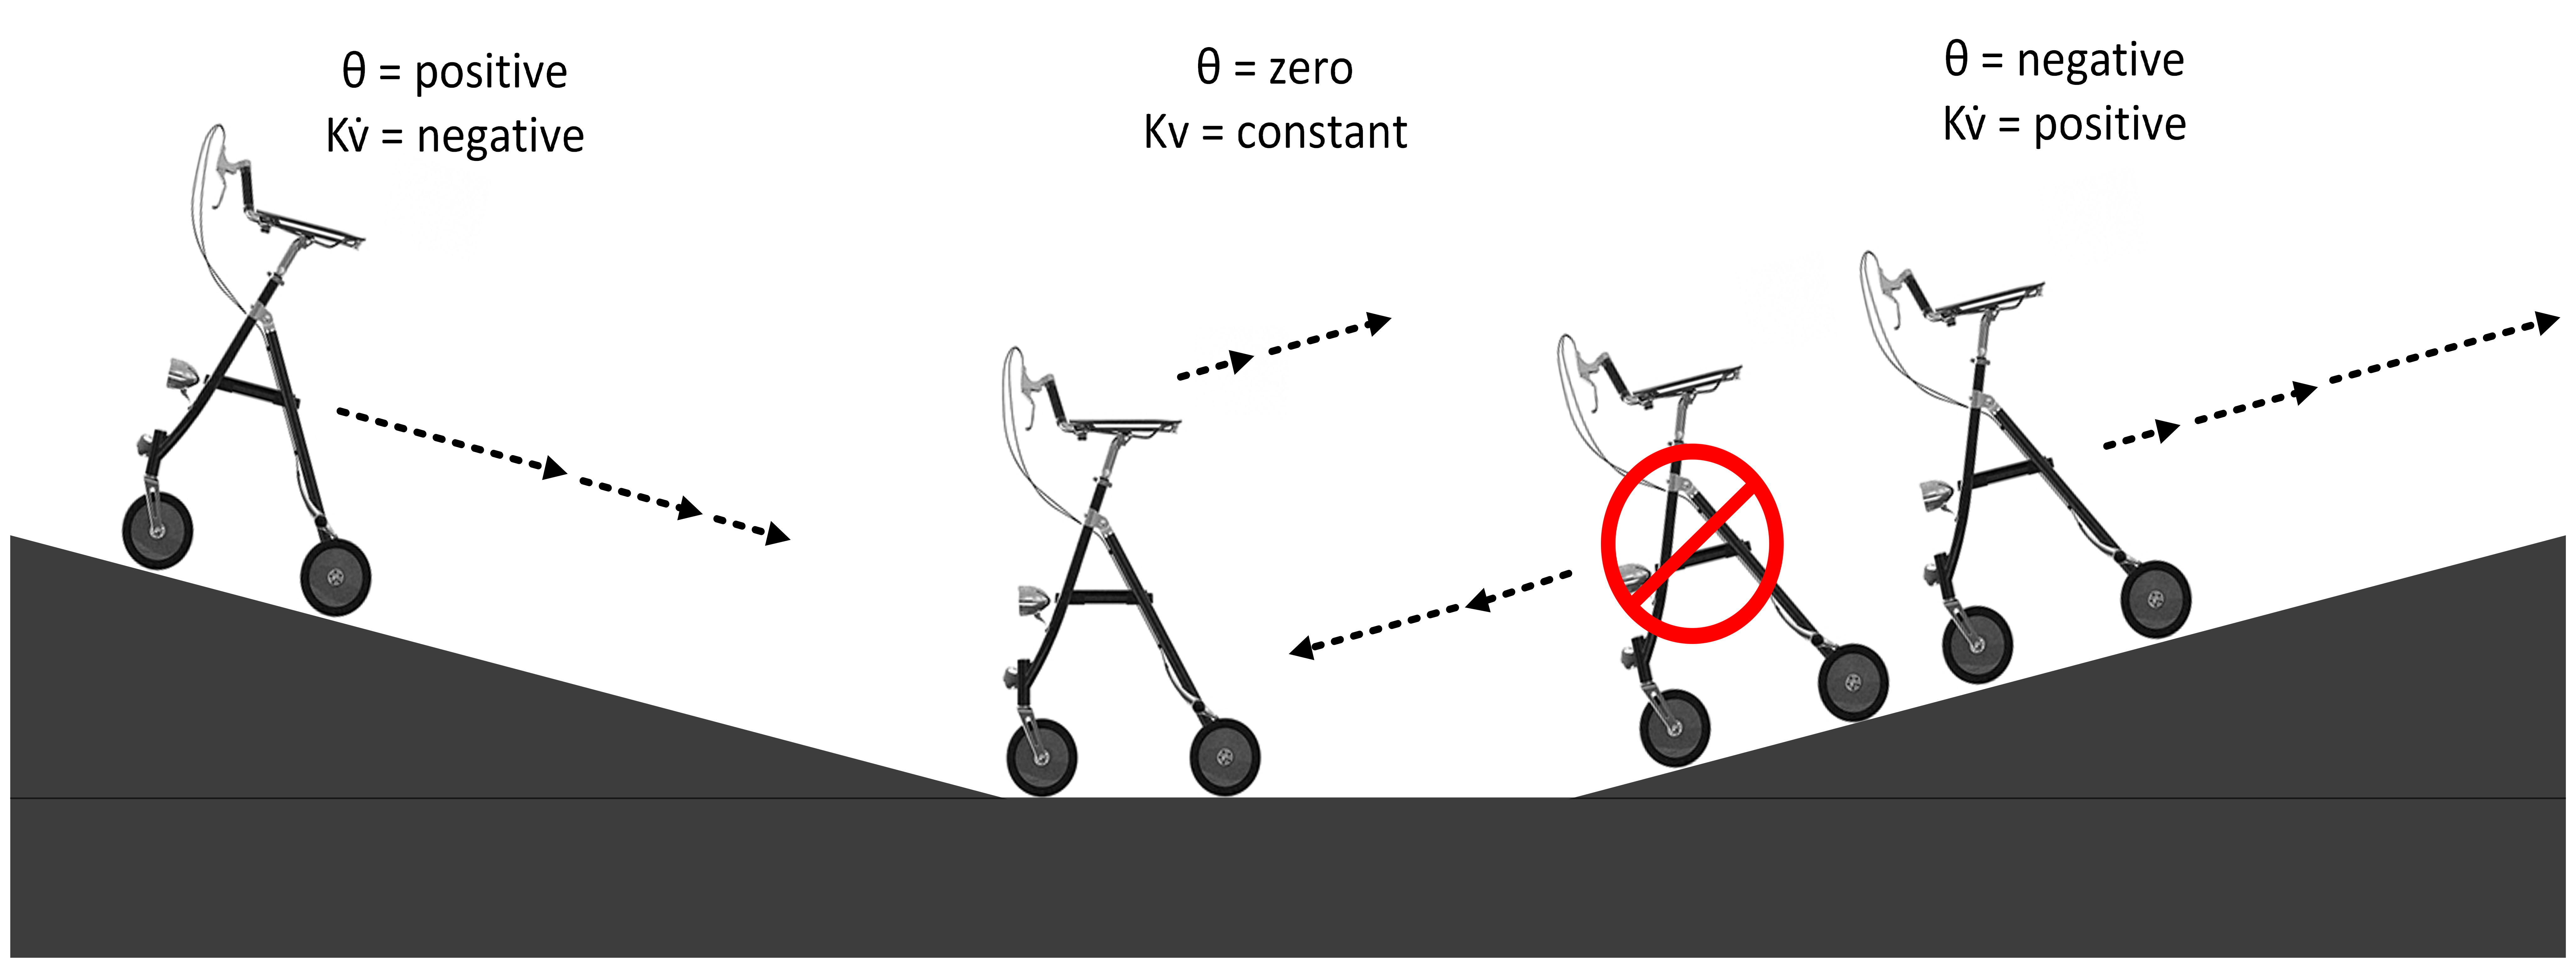
\includegraphics[width=\textwidth]{./Images/Incline-Decline-Stability.png}
	\caption{\label{fig:slope-stability}Stability on Slopes}
\end{figure}

\subsubsection{Sensor Fusion}
\noindent How do we make sense of the range detection made at all five points of the front-face of the walker? How do we combine that with pixel data of the corners of an object detection made by the camera? We can generally perceive depth by averaging the 4 coordinates, where closer is a higher average. We also know whether an obstacle is on the left or right side ahead based on which ranges are lower the maximum. We have to take into account the dead zones. With all of this information available on the network, we can build algorithms to guide the way forward, as discussed in the following chapter.\\

\noindent As noted, the ESP32 development board supports all the sensors and the camera simultaneously without the need of multiplexing. The setup pictured below in figure \ref{fig:bb-test} has the IMU and LiDAR on an I2C bus, and the ultrasonic sensors routed to GPIO pins. A table of the varying assignments, labels, and voltage requirements would be provided for the topology in figure \ref{fig:bb-test}, but it is forbidden by the UCF ECE guidelines. Suffice it to say, the IMU requires 3.3V, the TFLuna LiDAR requires 5V, and both variants of the ultrasonic can support either voltage.\\
\begin{figure}[H]
	\centering
	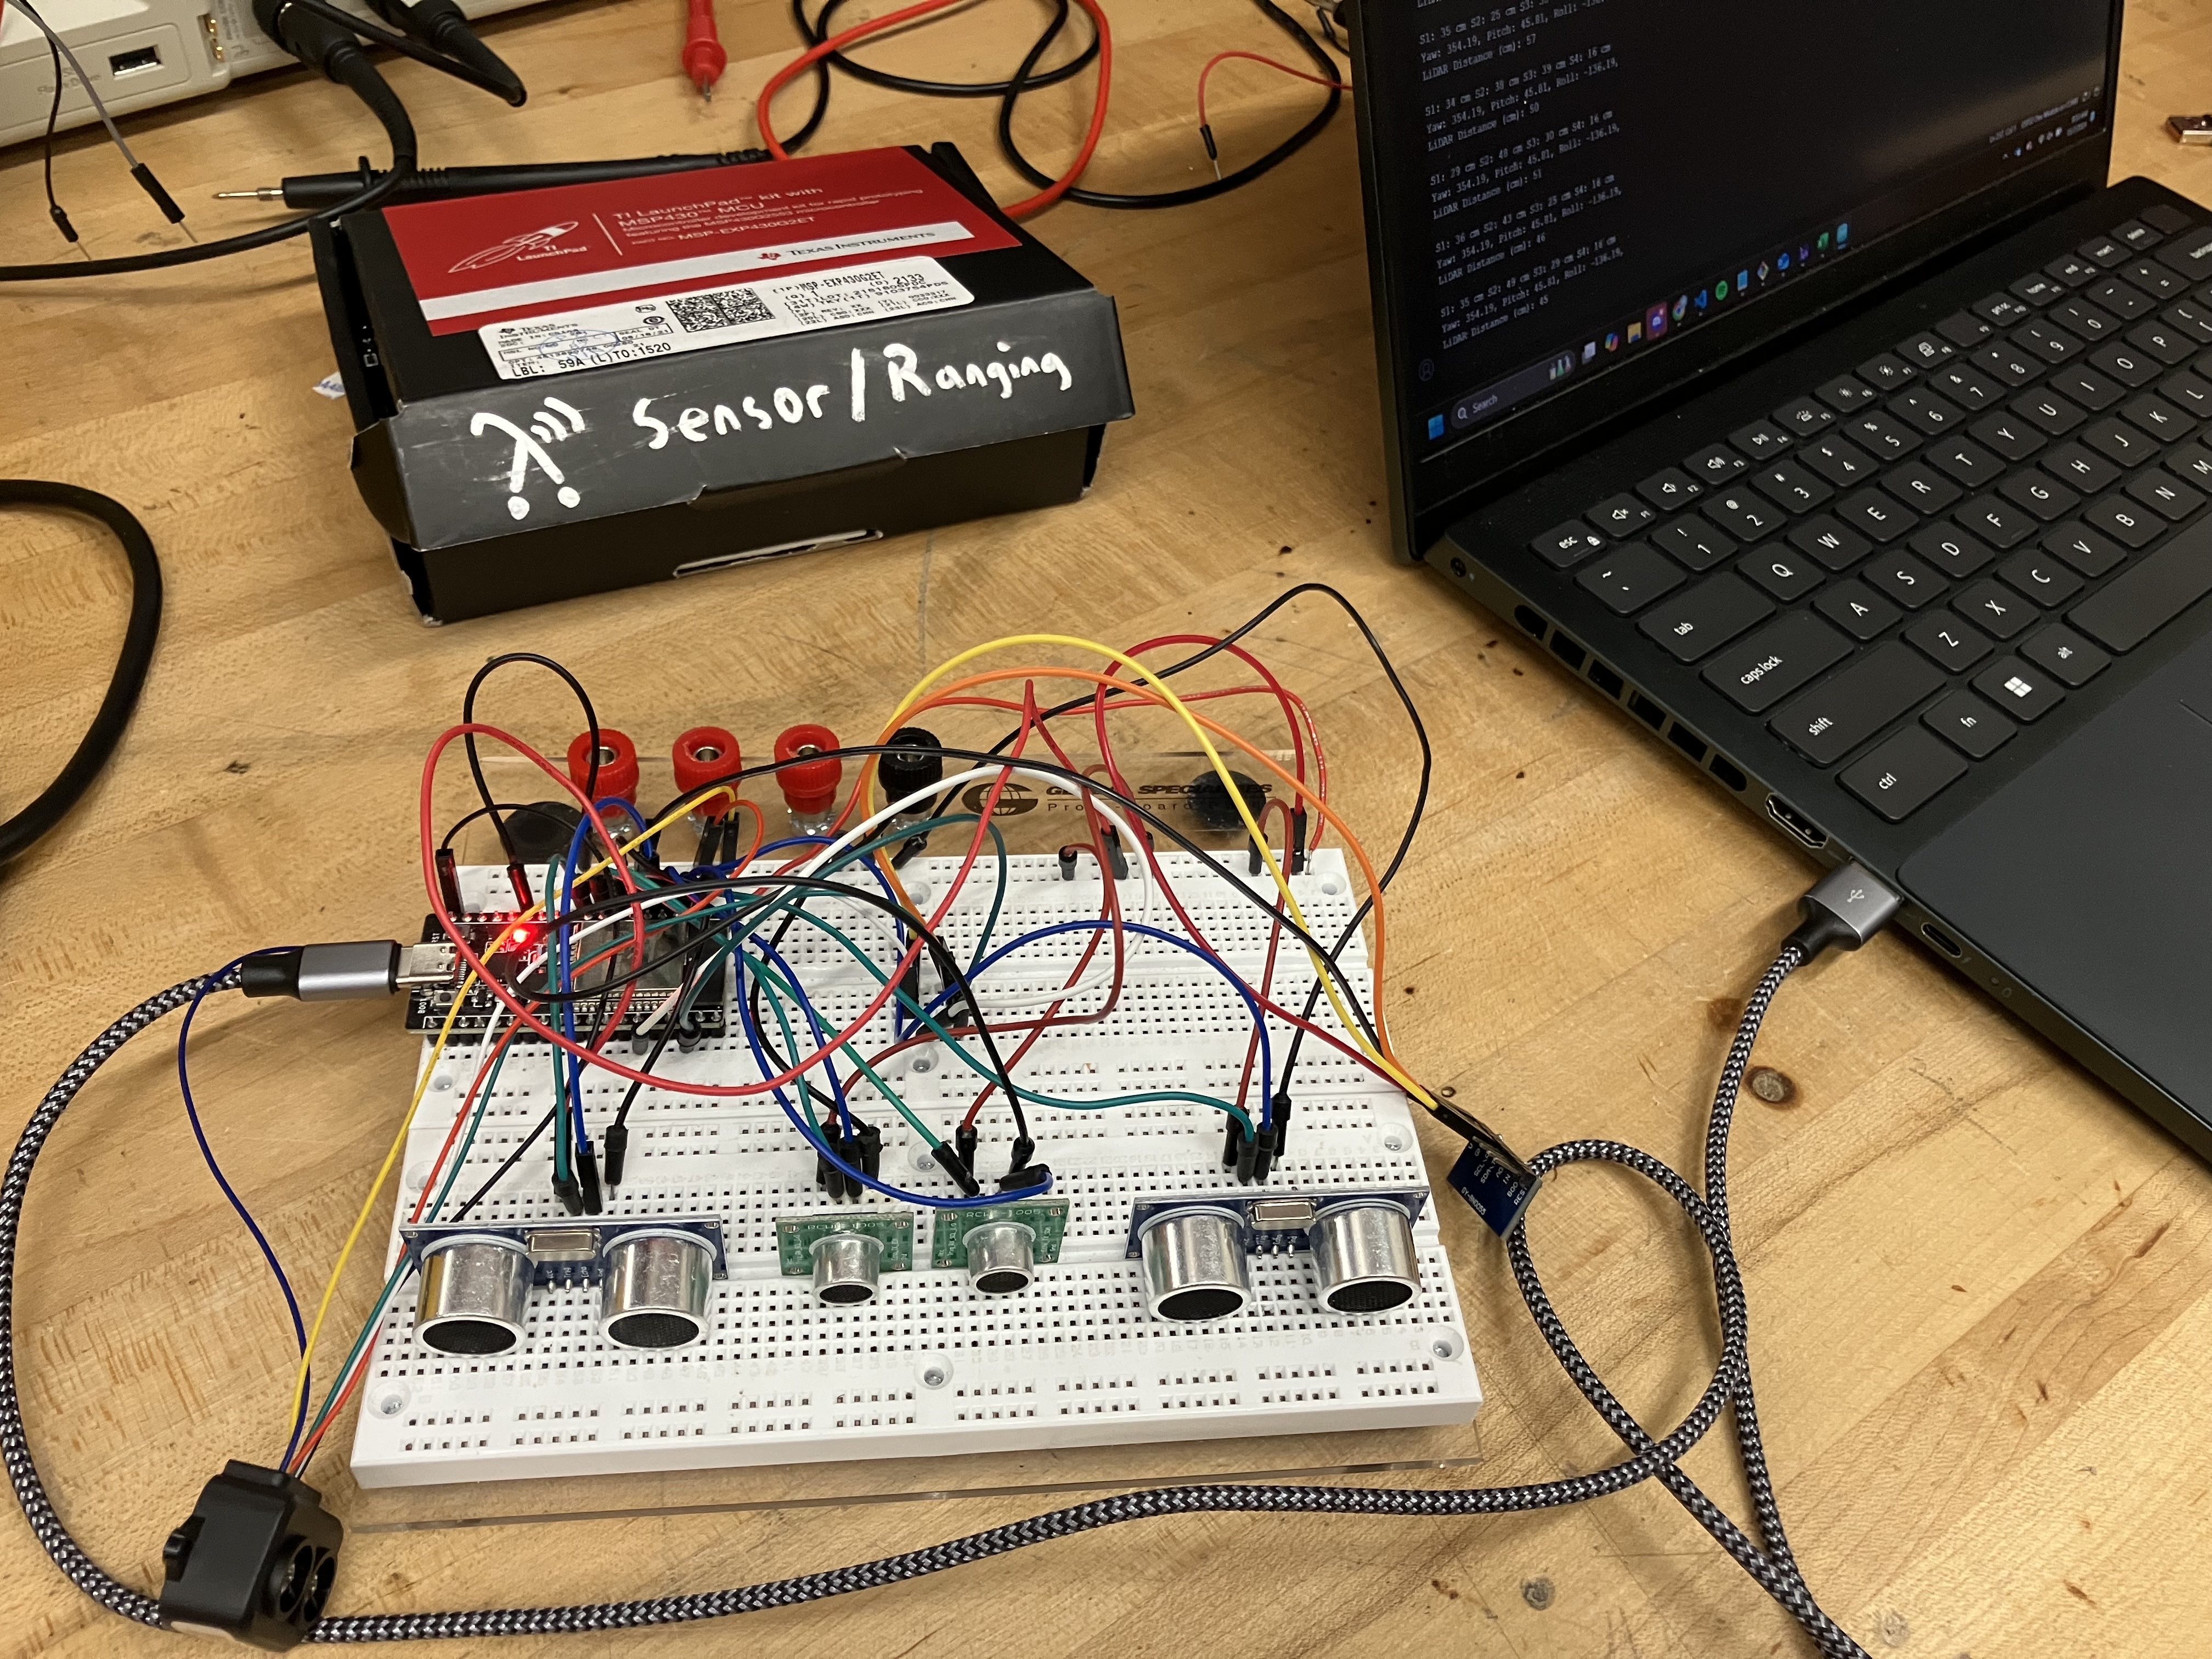
\includegraphics[width=0.5\textwidth]{./Images/breadboard-test.jpg}
	\caption{\label{fig:bb-test}Breadboard w/ Ultrasonics, and IMU \& LiDAR I2C Bus}
\end{figure}
